\section{Introduction}\label{sec:intro}

A core competency of many autonomous systems is to be aware of the state of
their environments so that they may operate safely in them. For example, an
autonomous vehicle needs to be aware of other cars on the road for a path
planning module to propose safe actions. This object detection task has been
extensively studied in the literature using different sensor modalities,
including camera imagery and \ac{LIDAR}.

However, object detection alone does not paint a complete picture of the
environment for the robot. It is also critical for a robot to make inferences
and decisions regarding where objects possibly \emph{could} be; for example, a
robot might need to ask ``how likely is it that a pedestrian is present in this
occluded region?" The answer to this question can be the difference between
driving through an intersection unhindered or cautiously anticipating a
pedestrian hidden behind a parked car.

\begin{figure}[!t]
  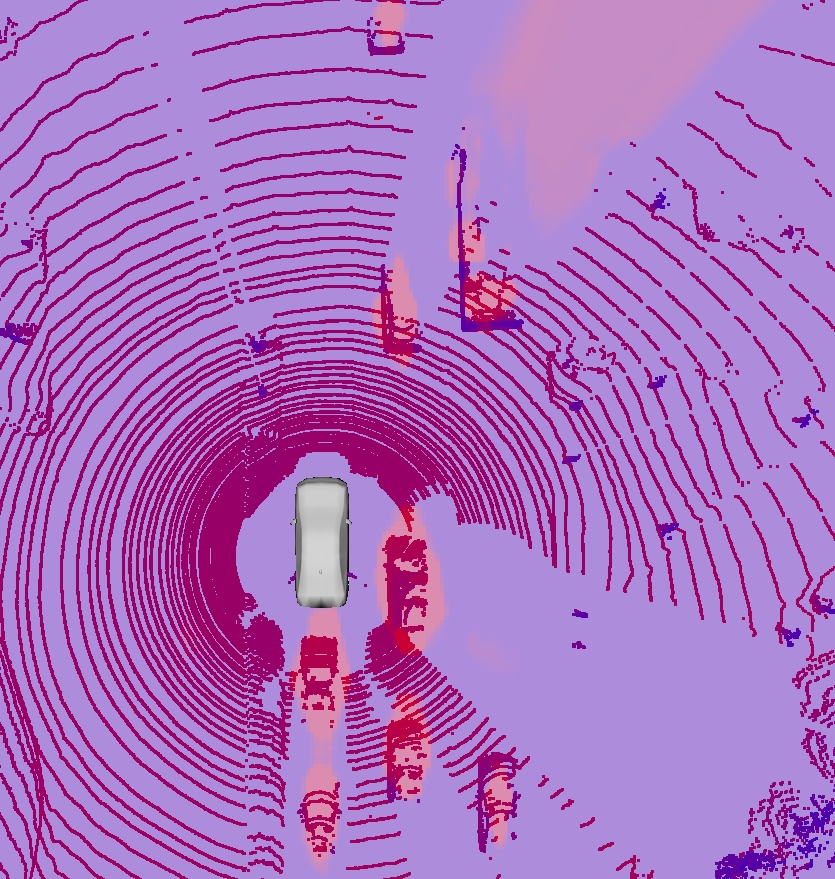
\includegraphics[width=\columnwidth]{figures/badge.jpg}
  \caption{A bird's eye view of sample output from our proposed system run on
    the KITTI dataset. Red colors indicate high probabilities for cars, blue
    indicates high probabilities for background. (Best viewed in color.) }
  \vspace{-7mm}
  \label{fig:badge}
\end{figure}

\figref{fig:badge} shows an example of a situation that an autonomous car might
encounter. In addition to detecting the cars present in the environment, we
wish to capture areas we know are absent of cars (shown in blue) or areas where
there might be cars that are hidden (such as the occluded region in the top
right).

The state-of-the-art in object detection, while performing very well in the pure
detection task, is ill-suited to answer these types of queries. These methods
typically do not fully model the nature of range-based sensors such as
\ac{LIDAR}, often using solely the points that are returned. Thus, there is no
way to differentiate between free and unknown regions of the world.

Occupancy mapping and related work is better suited for differentiating between
free and unknown space, as they explicitly model these. However, this mapping is
typically performed per voxel, and there is no notion of the potential absence
or presence of an \emph{object class}.

In this paper, we blend these two paradigms; we present a method that
consumes \ac{LIDAR} data and produces a probabilistic distribution of object-level
detections that can represent known objects in the world, areas were objects are
known to be absent, and regions of uncertainty. To achieve this, we rely on
techniques from both approaches, including ray-casting to sweep out free space
and the use of object-level observation models. Additionally, we formulate our
approach in a Bayesian framework, allowing for simple integration of additional
sensor modalities.

The goals of this work include:
%
\begin{itemize}
  \item Explicitly modeling occupied, free, and unknown space in a Bayesian
    formulation that is easily amendable to multi-modal sensing or temporal
    updates.
  \item Generation of a probabilistic detection map that can be queried at any
    location for the presence of a given object.
\end{itemize}
%
Additionally, we provide some preliminary results of this approach on the KITTI
dataset \cite{Geiger2013IJRR}.
